\documentclass[journal,12pt,twocolumn]{IEEEtran}
\usepackage{tikz-qtree}
\usepackage{subfiles} % Best loaded last in the preamble
\usepackage{setspace}
\usepackage{gensymb}
\singlespacing
\usepackage[cmex10]{amsmath}

\usepackage{amsthm}

\usepackage{mathrsfs}
\usepackage{txfonts}
\usepackage{stfloats}
\usepackage{bm}
\usepackage{cite}
\usepackage{cases}
\usepackage{subfig}

\usepackage{longtable}
\usepackage{multirow}

\usepackage{enumitem}
\usepackage{mathtools}
\usepackage{steinmetz}
\usepackage{tikz}
\usepackage{circuitikz}
\usepackage{verbatim}
\usepackage{tfrupee}
\usepackage[breaklinks=true]{hyperref}
\usepackage{graphicx}
\usepackage{tkz-euclide}

\usetikzlibrary{calc,math}
\usepackage{listings}
    \usepackage{color}                                            %%
    \usepackage{array}                                            %%
    \usepackage{longtable}                                        %%
    \usepackage{calc}                                             %%
    \usepackage{multirow}                                         %%
    \usepackage{hhline}                                           %%
    \usepackage{ifthen}                                           %%
    \usepackage{lscape}     
\usepackage{multicol}
\usepackage{chngcntr}

\DeclareMathOperator*{\Res}{Res}

\renewcommand\thesection{\arabic{section}}
\renewcommand\thesubsection{\thesection.\arabic{subsection}}
\renewcommand\thesubsubsection{\thesubsection.\arabic{subsubsection}}

\renewcommand\thesectiondis{\arabic{section}}
\renewcommand\thesubsectiondis{\thesectiondis.\arabic{subsection}}
\renewcommand\thesubsubsectiondis{\thesubsectiondis.\arabic{subsubsection}}


\hyphenation{op-tical net-works semi-conduc-tor}
\def\inputGnumericTable{}                                 %%

\lstset{
%language=C,
frame=single, 
breaklines=true,
columns=fullflexible
}
\begin{document}


\newtheorem{theorem}{Theorem}[section]
\newtheorem{problem}{Problem}
\newtheorem{proposition}{Proposition}[section]
\newtheorem{lemma}{Lemma}[section]
\newtheorem{corollary}[theorem]{Corollary}
\newtheorem{example}{Example}[section]
\newtheorem{definition}[problem]{Definition}

\newcommand{\BEQA}{\begin{eqnarray}}
\newcommand{\EEQA}{\end{eqnarray}}
\newcommand{\define}{\stackrel{\triangle}{=}}
\bibliographystyle{IEEEtran}
\raggedbottom
\setlength{\parindent}{0pt}
\providecommand{\mbf}{\mathbf}
\providecommand{\pr}[1]{\ensuremath{\Pr\left(#1\right)}}
\providecommand{\qfunc}[1]{\ensuremath{Q\left(#1\right)}}
\providecommand{\sbrak}[1]{\ensuremath{{}\left[#1\right]}}
\providecommand{\lsbrak}[1]{\ensuremath{{}\left[#1\right.}}
\providecommand{\rsbrak}[1]{\ensuremath{{}\left.#1\right]}}
\providecommand{\brak}[1]{\ensuremath{\left(#1\right)}}
\providecommand{\lbrak}[1]{\ensuremath{\left(#1\right.}}
\providecommand{\rbrak}[1]{\ensuremath{\left.#1\right)}}
\providecommand{\cbrak}[1]{\ensuremath{\left\{#1\right\}}}
\providecommand{\lcbrak}[1]{\ensuremath{\left\{#1\right.}}
\providecommand{\rcbrak}[1]{\ensuremath{\left.#1\right\}}}
\theoremstyle{remark}
\newtheorem{rem}{Remark}
\newcommand{\sgn}{\mathop{\mathrm{sgn}}}
% \providecommand{\abs}[1]{\left\vert#1\right\vert}
% \providecommand{\res}[1]{\Res\displaylimits_{#1}} 
% \providecommand{\norm}[1]{\left\lVert#1\right\rVert}
% %\providecommand{\norm}[1]{\lVert#1\rVert}
% \providecommand{\mtx}[1]{\mathbf{#1}}
% \providecommand{\mean}[1]{E\left[ #1 \right]}
\providecommand{\fourier}{\overset{\mathcal{F}}{ \rightleftharpoons}}
%\providecommand{\hilbert}{\overset{\mathcal{H}}{ \rightleftharpoons}}
\providecommand{\system}{\overset{\mathcal{H}}{ \longleftrightarrow}}
	%\newcommand{\solution}[2]{\textbf{Solution:}{#1}}
\newcommand{\solution}{\noindent \textbf{Solution: }}
\newcommand{\cosec}{\,\text{cosec}\,}
\providecommand{\dec}[2]{\ensuremath{\overset{#1}{\underset{#2}{\gtrless}}}}
\newcommand{\myvec}[1]{\ensuremath{\begin{pmatrix}#1\end{pmatrix}}}
\newcommand{\mydet}[1]{\ensuremath{\begin{vmatrix}#1\end{vmatrix}}}
\numberwithin{equation}{subsection}
\makeatletter
\@addtoreset{figure}{problem}
\makeatother
\let\StandardTheFigure\thefigure
\let\vec\mathbf
\renewcommand{\thefigure}{\theproblem}
\def\putbox#1#2#3{\makebox[0in][l]{\makebox[#1][l]{}\raisebox{\baselineskip}[0in][0in]{\raisebox{#2}[0in][0in]{#3}}}}
     \def\rightbox#1{\makebox[0in][r]{#1}}
     \def\centbox#1{\makebox[0in]{#1}}
     \def\topbox#1{\raisebox{-\baselineskip}[0in][0in]{#1}}
     \def\midbox#1{\raisebox{-0.5\baselineskip}[0in][0in]{#1}}
\vspace{3cm}
\title{Assignment 1}
\author{Krati Arela - EE18BTECH11050}
\maketitle
\newpage
\bigskip
\renewcommand{\thefigure}{\theenumi}
\renewcommand{\thetable}{\theenumi}
Download all latex-tikz codes from 
%
\begin{lstlisting}
https://github.com/Krati012/C-and-DS/tree/main/Assignment1
\end{lstlisting}
\section{Problem}
(Q. 20) The postorder traversal of a binary tree is 8,9,6,7,4,5,2,3,1. The inorder traversal of the same tree is 8,6,9,4,7,2,5,1,3. The height of a tree is the length of the longest path from the root to any leaf. The height of the binary tree above is \rule{1cm}{0.15mm}?
\section{Solution}
\textbf{Answer}: The height of the above binary tree is 4.
\newline
\textbf{Explanation}: \textbf{Postorder traversal} of a binary tree is a depth-first search in which we first traverse the left subtree, then traverse the right subtree, and finally visit the root node. Whereas in \textbf{inorder traversal} we first traverse the left subtree, visit the root and then traverse the right subtree.
\newline
If there are n nodes in binary tree, maximum height of the binary tree is \textbf{$n-1$}.
\newline
A complete binary tree will have minimum height for given $n$ number of nodes. Then height $h$ will lie in the range:
\begin{equation}
\label{eq:eqn1}
 2^h \leq n \leq 2^{h+1} - 1
\end{equation}
Thus, solving this inequality we get:
\begin{equation}
\label{eq:eqn2}
 h \leq log_{2}n,  h \geq log_{2}(n+1) - 1
\end{equation}
Since $h$ is an integer, we finally get,
\begin{equation}
\label{eq:eqn3}
 h = floor(log_{2}n) = ceil(log_{2}(n+1) - 1)
\end{equation}
Therefore, for a binary tree maximum height is \textbf{$n-1$} and minimum height is \textbf{$floor(log_{2}n)$}.
For given problem, n=9, so maximum height of the binary tree possible is 8 and minimum height possible is 3. 
\newline
The following algorithm allows us to construct the binary tree from given $inorder = [8,6,9,4,7,2,5,1,3]$ and $postorder = [8,9,6,7,4,5,2,3,1]$:
\begin{itemize}
    \item  First find the last node in postorder[], as root always appear in the end of postorder traversal. The root is "1" in this problem.
    \item  Search “1” in inorder[] to find left and right subtrees of root. Everything on left of “1” in inorder[] is in left subtree and everything on right is in right subtree. 
    \item Recur the above process for following two:
    \begin{itemize}
        \item Recur for $inorder = [8,6,9,4,7,2,5]$ and $postorder = [8,9,6,7,4,5,2]$. The created tree will be left child of root.
        \item Recur for $inorder = [3]$ and $postorder = [3]$. The created tree will be right child of root.
    \end{itemize}
\end{itemize}


\begin{figure}[!ht]
\centering
\subfile{tree}
\caption{Constructed Binary Tree}
\label{fig:bst}
\end{figure}
The following C code uses the above algorithm to construct the tree and prints the height of the tree as output. 
\begin{lstlisting}
    codes/height_bst.c
\end{lstlisting}
The constructed tree from above algorithm is shown in Fig. \ref{fig:bst}
\newline
Thus, we can see that the height of the tree is 4.

\section{Generating Order Array}
The following algorithm allows us to generate inorder and postorder traversal array for any given height h.
\begin{itemize}
    \item Initialize array of size $2*h + 1$ for inorder and postorder arrays.
    \item Initialize root of binary tree as 1 and recursively create child nodes of root with values as $2*(i+1)$ and $2*(i+1)+1$, with $i=0,1,..,h-1$.
    \item Insert the values of the nodes of the tree in inorder or postorder traversal as required in array and return the array.
\end{itemize}

The following code generates inorder and postorder traversal arrays for random binary tree for any given height.
\begin{lstlisting}
    codes/generate_order.c
\end{lstlisting}

To verify the algorithm, generate arrays for any height h, for eg, $h = 20$, and apply the function to construct and find height of binary tree in height\_bst.c, which gives height of the tree as 20.
Thus the algorithm is verified.

\section{Complexity}
The following code runs our program height\_bst.c for different values of n (which is the height of the tree) and saves the execution time in a text file. 
\begin{lstlisting}
    codes/run.c
\end{lstlisting}
\section{Solution}
Let us assume the time complexity to process the given input of size $n$ to be $T(n)$ and time taken to process input $n-1$ will be $T(n-1)$. Our program recursively calls the construct function for right and left subtrees. 
\begin{equation}
\label{eq:eqn4}
 T(n) = T(n-1) + n + C
\end{equation}
 We get eq \eqref{eq:eqn4} as in the worst case, search in inorder array will take $O(n)$ time, and $C$ is some constant time taken in the process.
\begin{equation}
\label{eq:eqn5}
 T(n-1) = T(n-2) + n + C
\end{equation}
Substituting \eqref{eq:eqn5} in \eqref{eq:eqn4},
\begin{equation}
 T(n) = T(n-2) + 2n + 2C
\end{equation}
On repeated substitution till $n->0$,
\begin{equation}
 T(n) = T(0) + n*n + nC
\end{equation}
\begin{equation}
 \implies T(n) = n^2 + nC + T(0)
\end{equation}
\begin{equation}
 \implies T(n) \leq n^2
\end{equation}
\begin{equation}
 \implies T(n) \in O(n^2)
\end{equation}
Thus, our program has $O(n^2)$ time complexity.
The given python file plots the time complexity using the execution time for different size of inputs.
\begin{lstlisting}
    codes/exec_time.py
\end{lstlisting}
\begin{figure}[!ht]
\centering
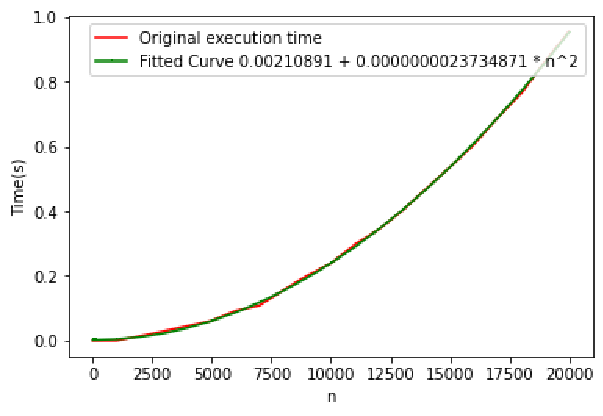
\includegraphics[width=\columnwidth]{./figs/plot}
\caption{$T(n)\: vs \: n$}
\label{fig:time}
\end{figure}
We can clearly observe that the original execution time and our mathematical time complexity align with each other.
\end{document}
